% Options for packages loaded elsewhere
\PassOptionsToPackage{unicode}{hyperref}
\PassOptionsToPackage{hyphens}{url}
%
\documentclass[11pt]{book}
\author{Fania Everitt}
\date{15/09/2021}

\usepackage{amsmath,amssymb}
\usepackage{lmodern}
\usepackage{iftex}


\usepackage{geometry}
\geometry{
 a4paper,
 total={170mm,257mm},
 left=20mm,
 top=20mm,
 }



% I-Ching stuff
\usepackage{fontspec}
\usepackage{xeCJK}
% \setCJKmainfont{LiSong Pro}
\setCJKmainfont{SimSun}
\newCJKfontfamily{\dejavusanszh}{DejaVu Sans} % this font has the required glyphs
\newfontface{\dejavusans}{DejaVu Sans} % this font has the required glyphs
\newcommand{\iching}[1]{{\dejavusanszh\char\numexpr"4DC0+#1}}
\newcommand{\trigram}[1]{{\dejavusans\char\numexpr"2630+#1}}


\usepackage{marvosym} % for yinyang symbol


% \ifPDFTeX
%   \usepackage[T1]{fontenc}
%   % \usepackage[utf8]{inputenc}
%   \usepackage{textcomp} % provide euro and other symbols
% \else % if luatex or xetex
%   \usepackage{unicode-math}
%   \defaultfontfeatures{Scale=MatchLowercase}
%   \defaultfontfeatures[\rmfamily]{Ligatures=TeX,Scale=1}
% \fi
% Use upquote if available, for straight quotes in verbatim environments
\IfFileExists{upquote.sty}{\usepackage{upquote}}{}
\IfFileExists{microtype.sty}{% use microtype if available
  \usepackage[]{microtype}
  \UseMicrotypeSet[protrusion]{basicmath} % disable protrusion for tt fonts
}{}
\makeatletter
\@ifundefined{KOMAClassName}{% if non-KOMA class
  \IfFileExists{parskip.sty}{%
    \usepackage{parskip}
  }{% else
    \setlength{\parindent}{0pt}
    \setlength{\parskip}{6pt plus 2pt minus 1pt}}
}{% if KOMA class
  \KOMAoptions{parskip=half}}
\makeatother
\usepackage{xcolor}
\IfFileExists{xurl.sty}{\usepackage{xurl}}{} % add URL line breaks if available
\IfFileExists{bookmark.sty}{\usepackage{bookmark}}{\usepackage{hyperref}}
\hypersetup{
  hidelinks,
  pdfcreator={LaTeX via pandoc}}
\urlstyle{same} % disable monospaced font for URLs
\usepackage{longtable,booktabs,array}
\usepackage{calc} % for calculating minipage widths
% Correct order of tables after \paragraph or \subparagraph
\usepackage{etoolbox}
\makeatletter
\patchcmd\longtable{\par}{\if@noskipsec\mbox{}\fi\par}{}{}
\makeatother
% Allow footnotes in longtable head/foot
\IfFileExists{footnotehyper.sty}{\usepackage{footnotehyper}}{\usepackage{footnote}}
\makesavenoteenv{longtable}
\setlength{\emergencystretch}{3em} % prevent overfull lines
\providecommand{\tightlist}{%
  \setlength{\itemsep}{0pt}\setlength{\parskip}{0pt}}
\setcounter{secnumdepth}{-\maxdimen} % remove section numbering
\ifLuaTeX
  \usepackage{selnolig}  % disable illegal ligatures
\fi


% for drawing extra Trigrams / Hexagrams
\usepackage{tikz}
\usetikzlibrary{arrows}
\usetikzlibrary{arrows.meta}

\tikzset{%
    % ->-/.default=.5%
  baseline=-0.5ex,
  % line width=.04cm,
  line cap=butt,%
  every picture/.style={line width=.04cm}
}





\begin{document}
\frontmatter

% \tableofcontents


\mainmatter

\chapter{THE I CHING (BOOK OF CHANGE)}

\emph{D. Everitt F/A III}


\section{Introduction}

The I Ching is not ordinary reading. It may appear to be a curious hybrid of superstition and `fortune' on one hand, and the most sublime and penetrating insight into human patterns on the other. It is a unity of planned and unplanned, or freewill and choice; destiny and duty, demonstrating as it does the intyerplay of these complementary factors. It elucidates a situation, leaving us responsible for further action. It carefully extracts the noble aspects of our character in such a way that we cannot help but heed its advice.

Whatever he says to the contrary, a man needs a superior if he is to improve his way of living. The I Ching serves as a guide, yet as a guide it constantly refers us to the ``superior man''-which is best realised as being within ourselves-and the ``great man'' or ``sage'' whose conduct is exemplified as being in accordance with `Tao'-the `way of heaven'. In using the I Ching, or investinating its principles, we have to accept that it seems to know better than we do; but in fact, it only extracts from within ourselves qualities we always possessed, but tended to overlook, primarily: `intuition'. In learning the language of the occurences around us, all of which have specific causes, we learn to read probable future occurences and also the most beneficial mode of behaviour for the present ones.

How it is achieved is an elusive point, but the I Ching always seems firstly to echo our own conscience or intuition of what is actually occuring, and secondly to be a step ahead of us. As long as we are operating from selfish motives and personality preferences, then we experience a latent anxiety as a defence against the removal or denial of our sources of satisfaction and security. This anxiety always tends to distort our viewpoint of the situations around us and the way of the possibility of losing something of what we are attached to, and we mould and bend our lives as well as cirumstances in efforts to ensure the maximum amount of that which we desire, forgetting that what comes easiest can be left to look after itself and what comes hardest is what needs most attention. In doing this, we become one-sided or empty in some inner areas, and this factor causes more anxiety as we attempt to avoid situations which threaten our stability in their prodding of the weakest `empty' spots in our character. This is a pitiful state for a human being to entertain, yet our whole society not only accepts it, but is even built around its perpetuation, and encouragement towards personal satisfaction of a selfish kind. Even alternative ways are frequently poised by their own mental bias, often developing over-reaction to the sensed `wrong', and lop-sided approaches to its solution. We have to shift our attention not from unnatural ways of living to what are considered externally more natural ways, but from selfish motivation to a rather more universal consciousness of man as a race, and our unselfish role in that race's life-and this, willingly. From this consciousness only, can any needed external change be affected. Now most of us `know' this already, but fail to act upon it-why? Because, perhaps, we cannot escape the nagging attachements to our personal security. Whatever we may think about detachmnent, until it is realised within us we will still feel anguish and distress on hearing views which `disagree' with ours or in seeing our most cherished possessions endangered. The I Ching gives a large hint on how we can begin to transcend the seemingly uncontrollable bind of self centered reactions towards all that happens to us. We don't follow it like a rule book; on the lowest level of interpretation it tells us what course is open to us for our best benefit. On the highest level it can lead us to choose the situations which will lift us out of the world of selfishness once and for all. It will never provide that situation for us, any more than it can live our lives for us, for you can take a horse to water\ldots; but it does make plain to use that there is a choice, a way, and that it is neither advisable nor necessary to harbour petty likes, dislikes and damaging enmities all our life, and that a broader vision can be attained if only we are prepared to drop the narrower one. Given if we consider ourselves to have a broad outlook our very assertion of open-mindedness displays a need for further expansion and inclusiveness.

In talking about the I Ching, one can only really discuss what it has lead one to do or what it has clarified in one's own mind-to talk about the book itself would be dry, for the book is dry if not put into practice-and when it is put into practice, it leads us to behave in ways encouraged by every sage who has lived. It is these ways (or rather, this way) which is the most important thing about the book. To discuss it purely on intellectual levels is like discussing food when one is actually starving. Bearing in mind the above, I can only describe how the I Ching reinforces certain attitudes in me. It may affect others more or less deeply, and although its influence is basically similar for all, it is only when one is living in complete `harmony with Tao' that it becomes identical for all persons using the book. The essay is an attempt to clarify the I Ching basic lessons. To quote Paul Reps in his introduction to `Zen Flesh, Zen Bones' ``Here are fragments of its skin, flesh, bones, but not its marrow-never found in words.''


\section{Structure and Interpretation}

\begin{quote}
  ``The ultimate frame of reference for all that changes is the non-changing''-Wilhelm
\end{quote}


\subsection{The absolute. T'ai C'hi. Tao.Te.}

The absolute is named T'ai C'hi. From T'ai C'hi, the primal undifferentiated course (T'ai C'hi = great primal beginning) all things arise. Some viewpoints recognise another principle named Wu C'hi (without beginning\footnote{this is an intelligent guess.}) which is represented by a blank circle, with T'ai C'hi as a secondary principle represented by the Yin/Yang symbol \Yinyang. What is known as `Tao' has many meanings, but we can consider it as representing T'ai C'hi as man relates and is related to it. Therefore it is also translated as `the way' of `Heaven' (or T'ai C'hi). Tao is T'ai C'hi in action, most notably in the life of a `sage'. Tao is the universal law to which change is subject. That the principle of Tao was misunderstood even in early China we can be sure, Lao Tzu finding a need to declare ``The Tao that can be expressed in words is not the real Tao''\footnote{`Tao Te Ching' Ch. 1}. Tao is also the name given to the correct coduct of any being, so we may even have the Tao of a fish or a soldier, (rather similar to `Dharma' in Buddhism-the purpose and duty of the individual.)

Overlapping some of the meanings of Tao is `Te' (pron. `Teh'\footnote{\emph{Tê} `virtue' Homophone meaning-to get. In Taoist usage = virtue of a thing (what it `gets' from Tao) i.e.~Tê is the nature of a thing, because it is in virtue of its `te' that a thing is what it is. In such works as the `Tao Te Ching', Te is used in its more conventional meaning, but still overlaps with the above. \emph{Conventional meaning}: `moral virtue', `bounty', `to be grateful', or `to be concious that others ought to be grateful to oneself'.})-or Tao as functioning in the mind of an individual; meaning the whole integrated man, functioning as a sort, with the transmuted personality as a subject; and the mind after all personal judgement has been transcended. Personal Te also stands for the virtue gained in such a state-both in the sense of a specific power (e.g.~the `virtue of healing') and in the sense of a moral quality, Lao Tzu defined Tao as `Te', when it was functioning in the individual, Confucious defined `Te' as moral virtue or power acquired by practice and perserverence. Both definitions agree; Lao Tzu allows the meaning to remain unapplied to any specific quality. Confucious simply defines what is needed for Te to arise in the individual, and states its tangible effects when it is functioning through that individual.


\subsection{The polar opposites or complementaries. Yin. Yang.}

\begin{quote}
  ``The first two trigrams (see table on page \pageref{table:trigrams}), the creative and the receptive (yin\& yang), are shown as representatives of the two polar primal forces. The aim is to explain that matter is the product of energy. The light and the dark energies. The interaction of these forces gives rise to matter-that is, the firm and the yielding. Matter makes up the form, the body, of all beings in heaven and on earth, but it is always energy that keeps it in motion. The important thing is to maintain connection with these divine forces of light''-Wilhelm
\end{quote}

The most easily observed function of Tao; in fact the prime cause of manifestation, and all movement (life); is change (`I'). This `change' arises when T'ai C'hi manifests by differentiating itself into the polar principles of Yin (submissive, female, etc) and Yang (active, male, creative, etc). These interact and combine with each other in varying degrees giving rise to various states of matter and substance in constant flux, for Yin and Yang never balance each other or remain static for more than a split second, for no sooner has Yang reached it's peak then it begins to transform itself into Yin-as in the process of birth, growth, decay, death or dawn, midday, dush, night. Yin literally means `cloudy' and stands for the dark, the principle that works from below upward, and Yang literally means `banners waving in the sun' signifying something which is shone upon, and is bright, and stands for the light, the principle that works from above downwards. Thos concept cannot be grasped by thought, being as it is the representation of the cause of all creation. If we don't recognise and know that cause within ourselves, we can never understand it outside, and men will call it a `mystery' or `unknowable', which it isn't. `Shiva' and `Shakti' are the equivalents (`power' and `peace') of Yang and Yin in Indian cosmology. `Shiva' is the inward breath in a man, focusing upon the point between the eybrows-the `seat of the soul' or location of consciousness in the life of a sage or saint. `Shakti' is represented by the outward breath, which returns to the solar plexus-the location of the consciousness of ordinary man-the central storehouse of material vitality. Breath is very significant in all religions, and especially in Chinese Taoist meditation, (see `Secret of the Golden Flower'\footnote{a Chinese manual on mediation. (See also: `Taoist Yoga' by Lu K'uan Yü)} trans. Wilhelm) representing as it does the cause of all creating in it's dual role. In the in breath, one focuses ones consciousness at the desired point, and aligns ones mind to the `one self'. The out breath radiates the resultant peace and floods the lower man with regenerative energy. I am including this in the hope that a more subjective grasp of the `idea' of `Yin' and `Yang' can be experienced, for there is little in us more basic than the breath.

In the I Ching, Yang is represented by a single line \tikz[baseline=-0.5ex]{\draw(0,0)--(0.3,0);}, and Yin by a \tikz[baseline=-0.5ex]{\draw(0,0)--(0.12,0);}\tikz[baseline=-0.5ex]{\draw(0.18,0)--(0.3,0);}. So therefore 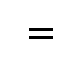
\begin{tikzpicture}[baseline=-0.5ex]\draw(0,0.1)--(0.3,0.1);\draw(0,0)--(0.3,0);\end{tikzpicture} represents the creative; 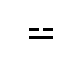
\begin{tikzpicture}[baseline=-0.5ex]\draw(0,0.1)--(0.12,0.1);\draw(0.18,0.1)--(0.3,0.1);\draw(0,0)--(0.3,0);\end{tikzpicture} and 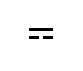
\begin{tikzpicture}[baseline=-0.5ex]\draw(0,0.1)--(0.3,0.1);\draw(0,0)--(0.12,0);\draw(0.18,0)--(0.3,0);\end{tikzpicture} represent states of transition, firstly with Yang predominantely (being the lower line of foundation, the upperbeing the outer expression of the lower-so Ynag here is expressing itself through a passive `personality' secondally with Yin ruling. 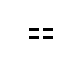
\begin{tikzpicture}[baseline=-0.5ex]\draw(0,0.1)--(0.12,0.1);\draw(0.18,0.1)--(0.3,0.1);\draw(0,0)--(0.12,0);\draw(0.18,0)--(0.3,0);\end{tikzpicture} represents Yin at its peak. If these lines are further combined in groups of three, we obtain the primal trigrams of King Wen (The word `Trigram' and `Hexagram'-one meaning a group of three; the other a group of six, lines; were used by Wilhem to replace `Kva' in Chinese, a figure composed of either three or six Kva)

\begin{longtable}[]{@{}
  >{\raggedright\arraybackslash}p{(\columnwidth - 4\tabcolsep) * \real{0.02}}
  >{\centering\arraybackslash}p{(\columnwidth - 4\tabcolsep) * \real{0.06}}
  >{\raggedright\arraybackslash}p{(\columnwidth - 4\tabcolsep) * \real{0.65}}
  >{\raggedright\arraybackslash}p{(\columnwidth - 4\tabcolsep) * \real{0.09}}
  >{\raggedleft\arraybackslash}p{(\columnwidth - 4\tabcolsep) * \real{0.12}}@{}}
\toprule
\endhead
\trigram{0} & Ch'ien & active, creative, strong, light, firm, cold, heaven & & Father \\
\trigram{7} & K'un & receptive, passive, `weak'\footnote{`weak' in the sense that although water is `weak', it wears away rock.}, dark, yielding, warm, earth & & Mother \\
\trigram{3} & Chên & thunder, movement, arousing, active, assigned to spring & eldest & Son \\
\trigram{5} & K'an & Abyss, water, dangerous, difficult, enveloping, winter\footnote{K'un is also assigned to winter for a reason too involved to explain here (K'an is the representative of K'un, sometimes {[}\ldots text indecipherable\ldots{]})} & second & Son \\
\trigram{6} & Kên & Mountain, hard, obstinete, immoreable, resting, keeping still & youngest & Son* \\
\trigram{4} & Sun & wood, wind, bland, mild, gentle, penetrating, flexible & eldest & Daughter \\
\trigram{2} & Li & fire, light, clinging, beautiful, depending, brilliant, clear & second & Daughter \\
\trigram{1} & Tui & lake, marsh, rain, joyful, satisfied, tranquil, complacent & youngest & Daughter** \\
\bottomrule
% \caption{Trigrams}
\label{table:trigrams}
\end{longtable}

* varying states of movement\\
** varying states of devotion\\
(I have by no means listed all the qualities or correspondances)

Ch'ien and K'un are regarded as the father and mother with the various trigrams as their sons and daughters, whose sex is determined by the numerical value of the lines. (Therefore, Li, for instance, represented by \trigram{2}, is female, although it contains two male lines and only one female one, because a male line is represented by the number 7 and female lines by 8. So 7 + 7 + 8 = 22, and all even numbers are female, according to this system.) Combining these trigrams of three lines in pairs, we obtain 8 x 8 permutations, or the 64 hexagrams, beginning with Ch'ien, made up of six male lines and K'un the receptive, of six (broken) female lines. These occur an equal number and symmetrical spacing combined, of both types of line in four notable hexagrams-number 11-T'ai-peace, consisting of 3 light lines resting upon 3 strong ones (light in weight that is) \iching{10}; and 12-P'i-stagnation, made up of \iching{11} or 3 heavy lines upon 3 weak ones. Then there are two hexagrams which complete the cycle, hexagrams 63 and 64-`after completion' and before completion, the hexagram 63 has all lines in corresponding strong or weak places (the place occupied by the bottom line of a hexagram is the first-number 1-and is strong, the second is weak and so on) signifying matters in transition from peace (-the culmination of movement) to standstill or stagnation-or, matters as they are after reaching completion. 64 has all lines in their correct relationship to one another, but not yet in their appropriate external place (so a yielding line occupies the first place; an active line, the second, passive, place: \iching{63}) signifying the transition from standstill or stagnation to peace-matters as they are `before completion'. The plain and broken lines represent the basic polarity and mutual complementary opposition of all phenomena. In their six positional values (from bottom to top of a hexagram) they show relativity in sequence of time and relationship in space.


\subsection{Arrangments, cycles, mathematics}

The varied cycles that the trigrams and hexagrams depict are adequately dealt with in already existing translations. The primary one is the cycle of a year as apparent in the seasonal cycle. The book itself is a cycle of another kind, beginning with undifferentiated positive and negative, and ending with the equal distribution of positive and negative lines, alternatively arranged (63 \& 64). Another sequence of arranging the hexagrams in a circle follows a binary system from 0 \iching{1} to 63 \iching{0} signified by K'un and Ch'ien (the binary system was derived by giving each line the value of a 0 for a Yin line, and a 1 for a Yang line so that ䷺ for instance, would read from the top downwards: 1 1 0 0 1 0 giving the value of 19). It is wrong to consider these cycles as independent from either the text or each other, since the interpretation of the hexagrams is derived from the interplay and combination of the meaning of the trigrams both primary and nuclear\footnote{see Interpretation}, and the hexagrams, in their various placements in the many arrangements and sequences. The cycles are determined by following the pattern of progression through certain lines or trigrams from stage to stage, and their correspondent meanings as they combine to form hexagrams. The Chinese undoubtadly saw the numerical as being integral with the symbolic. All of the I Ching can be found to have a mathematical or numerical basis, although mathematics is not here considered as an independant complex of abstract concepts, but is applied to things in a direct manner, rather than being self-referential. The aforementioned binary arrangement displays an interesting factor-the hexagrams opposing each other in the circle are the complementaries of each other (so \iching{46} would appear opposite \iching{21}, for instance). Succeeding hexagrams in the book sometimes restore themselves into their opposites: 27 (\iching{26}) is followed by 28 (\iching{27}), but often follow more obscure transformations.

It is logical, but I have never seen it mentioned, that all hexagrams, when their nuclear trigrams are combined with each other (the nuclear trigrams consist of the four inner lines, separated into 2, 3 and 4, and lines 3, 4, 5 - giving two new trigrams, thus the nuclear trigram of \iching{49} are derived by talking the four central lines and then splitting them, counting 3 from the bottom \trigram{0} and then using 3 upper lines \trigram{1} giving the two `nuclear' trigrams) resolve into either hexagrams 1 or 2, or 63 and 64, either directly, or by obtaining the further nuclear trigrams (following the above example; the obtained nuclear trigrams were \trigram{0} and \trigram{0} which give \iching{42} when combined, lower and upper being in correct places. The nuclear trigrams of \iching{42} are \trigram{0} and \trigram{0} again, giving \iching{0} or hexagram 1. This is not standard practice, as far as I know, but I consider it quite significant.) There are 12 hexagrams which resolve directly into 1, 2, 63, or 64.


\subsection{Interpretation}

According to the result gained from diving the yarrow stalks or throwing the coins, (ways of consulting the oracle\footnote{the exact processes are outlines in translations of the book.}) one will obtain a hexagram with or without `moving' lines-the moving lines are Yin or Yang lines which have beome `old' and are about to change into their opposites, to produce another hexagram. (Moving lines are signified by \begin{tikzpicture}[baseline=+1ex]\draw(0,0.325)--(0.3,0.325);\draw[line width=.02cm](0.15,0.325)circle[line width=.02cm,radius=0.035cm];\end{tikzpicture} for a Yang about to turn Yin, and \begin{tikzpicture}[baseline=+0.2ex]\draw(0,0.13)--(0.12,0.13);\draw(0.18,0.13)--(0.3,0.13);\draw[line width=.02cm](0.13,0.165)--(0.17,0.0925);\draw[line width=.02cm](0.17,0.165)--(0.13,0.0925);\end{tikzpicture} for Yin about to turn Yang. Thus the hexagram 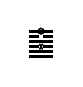
\begin{tikzpicture}[baseline=+0.1ex]\draw(0,0.325)--(0.3,0.325);\draw[line width=.02cm](0.15,0.325)circle[line width=.02cm,radius=0.035cm];\draw(0,0.26)--(0.12,0.26);\draw(0.18,0.26)--(0.3,0.26);\draw(0,0.195)--(0.3,0.195);\draw(0,0.13)--(0.12,0.13);\draw(0.18,0.13)--(0.3,0.13);\draw[line width=.02cm](0.13,0.165)--(0.17,0.0925);\draw[line width=.02cm](0.17,0.165)--(0.13,0.0925);\draw(0,0.065)--(0.3,0.065);\draw(0,0)--(0.3,0);\end{tikzpicture} would change into \iching{33}, when lines 3 and 6 completed their transition.) This gives 64 x 64 = 4086 possible answers to our enquiry. Anyone of the 64 hexagrams may change into any other one in this manner. When obtained, the many lines are read as part of the reply to the enquiry, and they usually point to particular details or exceptions to, and developments from, the main text of the hexagram. The \emph{nuclear trigrams} are important factors in the derivation of the symbolic texts also, reading through the hexagrams before and after the obtained will give us an idea of the causes for the present situation (indicated by the previous hexagram) and their likely outcome if events continue unmodified (indicated by the following hexagram). The line to which all other lines in the hexagram are subordinate is called the `ruling line', and often lies in the 5th place, or the 2nd, being central to the upper and lower trigrams, respectively; although the `ruling line' may occupy any of the 6 places, depending upon its purpose and the importance of the place. (- for instance, \iching{23} has line one as its ruler because it carries the theme of the hexagram `Return'-the returning of the creative principle from below).

The bottom trigram (or lower 3 lines) of a hexagram is within, below, behind and/or nearest to earth. The top 3 lines or trigram is outside, above, infront and/or nearest to heaven. The lower lines in general are the earliest in time. The bottom 2 lines signify earth; the next 2, man; the top 2, heaven; although a money line is the 5th or 6th place is not always favourable, since its position maybe inappropriate to the meaning of the whole hexagram (see p.361, Wilhelms translation). Since the 1st, 3rd and 5th are Yang; and the 2nd, 4th and 6th, are Yin, places, the `suitability' of a line in the hexagram depends upon its correctness in its passive or active place, accoring to the needs of the situation (see p.~358/9, Wilhelm). Line one, at the bottom, signifies not yet having fully entered into the matter, and line six indicates the opposite; having transcended or passed through the matter-often symbolised by a `sage' who stands above the worlds changes. Line six can also mean an extreme over-development of the rest of the hexagram (line 6 in the first hexagram, Ch'ien, signifies an `arrogrant dragon' \{the symbol of Ch'ien in general\} who `will have cause for repent'-the Confucian commentary adds: ``Arrogance means that one knows how to press forward but not how to draw back, that one knows extistence but not annihilation, knows something about winning, but nothing about losing. It is only the Holy man who understands how to press forward and how to draw back, who knows existence and annihilation as well, without losing his true nature.'' This arrogance is an over-developed power of the creative; a man who has ``risen so high that he has lost touch with the rest of mankind''.)


\subsection{Symbolism, Imagery}

\begin{quote}
  ``Straighforward words seem paradoxical''-Lao Tzu (LXXVIII)
\end{quote}

There are two symbols forming the I Ching; the basic lines, and their accompanying explanations. The lines are independent of language and although the interpretations given them depend partly upon the Chinese language and its associations, they are themselves universally applicable, and provide a skeleton upon which our creative perception may mould its insight. Most of the textual symbols depend upon understanding of Chinese life and its relation to the language and landscape, but even these are easily understood and applicable when seen in context and applied to Western life, since they symbolise basic moral, behavioural and psychological traits common in all civilizations. The apparently deep and veiled symbolism turns out to be quite straightforward, and it is seen at once that the original text was designed to speak directly to the subconscious(?) through familiar symbolism. When we are familiarised with its `obscurity', the symbolism has the same effect on us as it did to the Chinese mind. All symbols apply to man and macrocosm simultaneously, and the correspondance between the man in harmony with Tao and Tao itself is an important theme in the I Ching. The symbols transmit to us from the point of view of a sage; the detached onlooker-our own super-conscious or `soul'. Any interpretation is only a guideline-it may not wholly convey the meaning of the hexagram as it applies to our particular situation, for the Chinese language presents a difficulty in translation, having no gender or number (`he' might be `she'; `journey' might be `journeys'), however, the accompanying text will always furnish the fundamental trend of the hexagram, and usually proves quite adequate. A reading which does not seem to explain the hexagram in words appropriate to our actual conscious situation (although this only occurs rarely \{with me, anyways\} often yields a richer intuitive symbolism of the matter by virtue of its by-passing our conscious and clumsy grasps at immediate and obvious application of the words to our situation; perhaps allowing us to sense and understand some hitherto hidden factor. One begins to appreciate the value of parable and simile.

On consulting the Oracle, the `great treatise'\footnote{The main work in the I Ching. Included in Wilhelm's translation.} says: ``When the superior man is about to take action of a private or public nature he refers to the oracle, making his enquiry in words. It receives his messages, and the answer comes as if it were an echo. Whether the subject be far or near, mysterious or profound, he knows forthwith what its outcome will be.'' The `echo' of the oracle reveals our own position and nature all the more searchingly because it provides us with a means of becoming detached from our situtaion and our reaction to it. Further qualities desirable for correct interpretation are listed: absence of longing for the answer, receptivity and acceptance of what is given, and a still mind, -all pointing to a balanced, unbiased outlook. If the oracle is indiscriminately or lazily used, the enquirer loses his power to interpret the answer. In other words, it is useless to consult the oracle if we have not already done our utmost, and are not persisting in that effort-in such a case the I Ching may bring a suprised smile to our face by ``ticking us off'', especially if we have glossed over earlier readings! One can be excused for seeing the book as an entity with actual intelligence, if one has been the subject of such private humiliation! Blofeld in his forward, states: ``like Jung, I have been struck by the extraordinary sensation aroused by my consultations of the book, the feeling that my question has been dealt with exactly as by a living being in full possesion of even the unspoken facts involved in both the question and its answer (\ldots.) If you say that the oracle owes its effectiveness to the subconscious of the one who asks the questions, or to the unconscious, or to the One Mind, or to God or a God or the Gods, or to the philosophers Absolute, I shall be inclined to argue with every one of these suggestions.''

If we are reasonably unselfish and humble enough to admit that we can benefit from the work of many enlightened minds and lives, and we have a sincere desire to better our approach to, and insight into, circumstances confronting us, then we will certainly gain from a study of the guidance offered through the I Ching.


\section{History and Origin}

\begin{quote}
  ``In ancient times, when Fu Hsi ruled all things under heaven, he looked up and contemplated the bright patterns of the sky, then looked down and considered the shapes of the earth. He noted the decorative markings on birds and beasts, and the appropriate qualities of their territories. Close at hand he studied his own body, and also observed distant things. From all this he devised the eight trigrams, in order to unveil the heavenly processes in nature, and to understand the character of everything.''
\end{quote}

The above passage, taken from a commentary on the I Ching describes the steps taken in recording the patterns detected by man in nature and from which the I Ching stems in its original form. Fu Hsi, although regarded as legendary, is the first recorded Chinese Emporer (2852-2738 BC), and he is traditionally identified as the deviser and discoverer of the eight trigrams. However, the practice of casting oracles long antedates the formation of the I Ching. The oracles produced in heated sacred bones and tortoise shells (tortoises are a sacred and symbolic Chinese animal) were in general use as oracles long before and during the given time of Fu Hsi; and this practice must have combined with his (and others?) insight to produce the more ordered and advanced forms of the eight trigrams. In fact, one account explains the discovery of eight sacred symbols on the back of a sacred tortoise. In these two factors-the existing oracular practices, coupled with the inspiration of `Fu Hsi', we probably see the basic origins of the emergence of the I Ching as an ordered and recorded methodical system.

During an imprisonment, ``King'' Wen (a feudal lord of about 1150 BC-`King' is a posthumous title-he is often referred to as `King Wen' in the later commentaries) combined the eight trigrams of Fu Hsi in their sixty-four possible ways to produce the hexagrams, and added a name to each one, coupled with an explanation text. Forty years afterwards, his son, known as Duke Chou, expanded his father's work by adding a text appending to each separate line of every hexagram. Together, these two works constitute the basic text. Confucious (2500 BC)-who used his own copy so frequently that he wore through the leather thongs binding the tablets together, three times; and who said that if he had his life again, fifty years would be devoted to study of the I Ching-may have added parts of the commentaries on this text, but it is generally thought that his disciples added the main body of commentaries after their master's death.

In addition to these texts and their commentaries, which together make up the body of the I Ching as it exists today, there is a separate collection of added commentaries-known as the `great treatise'-not included as part of the I Ching, but usually read in conjunction with its deeper study. (Wilhelm's translation includes this latter work).

If Confusious was accurate in declaring the book ancient at the time of his own life, then the I Ching must have been in use in book form for at least 3000 years, and possibly even 4000, if we take Fu Hsi (or at least his dates) as literal; which makes it one of the oldest books in the world still in active use. At the time of the Meiji restoration in Japan, military tactics were based upon the patterns laid down in the I Ching, and in the earlier part of WW2 it was required reading for the higher ranks of Japanese officers. However, up to the present time it has undoubtedly been used by many of the general population including since the Western translations; a surprinsing number of people in the West; and its more noble use as a cosmological oracle and a system of patterns in life has been the study, together with Confucious, of many Chinese intellects.

The I Ching antedates the emergence of both Taoism (founder Lao Tzu? 500 BC) and Confucianism as distinct bodies of influence, but contains material which certainly furnished and fertilised the formation of both of them as external philosophical systems. (Their founder however, probably merely used existing philosophies to illustrate \& prove certain points, which were later elaborated and even held to constitute the actual `teachings' of those founders) Confucian influence in the I Ching tends towards the practical, political and human side of codes of conduct etc., while Taoism stresses the divine basics lying as a background to the oracle. Most of the common symbols are probably Chinese allegories of long-standing tradition, antedating even the I Ching, and I would consider that concentrating on the influences of any one external philosophy upon another is rather misleading, since they all are merely forms of expression for some inner experienced reality, the human subject of which used the existing systems and philosophies in an attempt to convey something of their experience to others. The merging of systems appears to be a natural process of their ageing, if barriers are not set up between them, since they tend to revert to what was already existing in everyday life after adding their own particular contribution to the society. The real initiator of influence to the actual experience which they attempt to describe (of Tao-`the way', and so on-all being the same experience, since religion in its true sense, is inclusive and synthetic) which is too easily overlooked when concentrating on the superficial interpolination of external doctrines and expressions. The Chinese approach to religion tends to be synthetic anyway, observing no barriers between the influence of Buddhism, Taoism, Confucianism or any other system and producing a pleasing, inclusive whole.

If we ignore earlier, obscure and often inaccurate attempts at European translation, the first truly sympathetic treatment of the book in the West was by Richard Wilhelm, backed up by a brief and confident foreword by Carl Jung, who praised its qualities as an oracle, and after having experimented and tested it extensively, who found it to reflect his own deeper mental processes in a remarkable way. Jung re-asserted the oracular and spiritual qualities of the I Ching, misunderstood by the West and even derided by one of the earlier translations (James Legge).


\subsection{Lessons from the I Ching}

Rather than presenting the concept of an eternal, changeless reality existing over and above a material world of lower value, the I Ching brings to light the eternal principle, immanent and operating through the medium of change in the material world. Time and change are two factors necessary to the existence of the world. In observing their patterns and interplay, we learn a great deal on how to live harmoniously; when to act and when to be still. We learn to utilise the prevailing currents instead of vainly trying to redirect them in attempts to make them conform with our own emotionally-biased wishes and plans. Time and space cannot be transcended as long as we remain selfishly-centered beings, although by altering our consciouness of them, we may witness apparent distortions. The whole key to harmonious living (whether circumstances or experiences be `good' or `bad') is to move with the moment-``for there is no external goal save that of the moment''-the external factor of time is the elusive `now', and of space is the `here': the `here and now'. By placing ourselves in the awareness of `here and now' we are able to grasp the opportunity of the moment and determine our future intelligently by acting upon the pattern uncovered by the present. However, in order to see this pattern, we need to stand aside and apart from our usual self-centered and self-oriented consciousness of everyday life. The I Ching is a subtle key towards helping us attain the balance needed for such a consciousness: ``The I Ching combines intuition and experience with a logical method of applying both to a given situation, which allows us to exert our reason (as a safeguard against a merely emotional approach or''wishful thinking'') and gives us the freedom as well as the responsibility of a fine decision. It is this that raises the I Ching to the level of a spiritual science and a philosophy of life and distinguishes it from a mere system of soothsaying or fortune-telling, in which man is deprived of his free will and conceived as a play-ball of fate, going to a pre-determined future, upon which he can have no influence.''\footnote{Lama Anagarika Govinda (from Blofeld's translation)}

In order to receive or achieve a vision of perfection, we first need to learn how to take advantage of factors presented in our more mundane lives. We do not jump from the self to the universal in one revalatory leap. We have to prepare the way at each single step, if our progress is to be permanent. To prepare the way, we have to be able to see it with sufficient detachment so as to avoid any distortion of the facts. Now everyone lives under certain illusions, which serve to limit our consciousness to a safe boundary until we are fit to cope with wider horizons. To remove these illusions prematurely is a sure way of causing gross imbalance or insanity and faneticism. Before the illusions disolve, we must be prepared; indeed, it is by the very act of preparation that we precipitate the dissolution of the barriers.

This fact is often ignored. We are all to eager to press for a sudden change or revelation, but rather shy of gradual but sure work produced by step for step progress, giving a balanced, progressive expansion. It is a common sight to see attempts at barrier-breaking by misunderstood, misapplied and inappropriate mystical, disciplinary and one-sided practises (as well as the common usage of drugs) and externally by social, political or economic means. Any barrier prematurely removed will almost certainly re-assert itself with more vehemence \& stubborness than before, when the factors released by breaking down that barrier are adequately handled. The fanaticism and dogmantism of most religions and political means is a prime example of this problem, yet the sincerity cannot be doubted. It is the very handling of day to day affairs that the I Ching deals with. It concerns arranging our methods to suit the available material.

Change is not bound to concealing the changeless, for it can be utilised as a `lever' whereby the changeless can be approached. The process of approach in itself, is simple, but as Lao Tzu stated: ``My words are very easy to understand and very easy to put into practice, yet no-one in the world can understand them or put them into practice''\footnote{`Tao Te Ching' Ch. LXX}-because it is against the grain of the degenerate form of human nature to act in accordance with `the way'. ``What comes easiest can be left alone; what comes hardest is that which needs most work'' is a phrase that is well-known among Kabbalists, and it applies equally well to all facets of life and progress. However, when we are threatened by a crisis, then fear of losing what we most appreciate spurs us on with admirable (if selfish) spirit! A crisis can be intelligently used as an opportunity to face that with which we are unfamiliar. This conflict can be seen as an opportunity to attempt to transcend our preferences in favour of a more impartial and inclusive approach, thereby lessening the possibility of anxiety caused by disliked and unfamiliar circumstances. In choosing to face such confrontations to our personality, we cultivate inner strength and stablity, and `moral virtue'. In such a way can change be used to approach an understanding of the changeless, for it displays to us any one-sidedness in our nature of approach to life, provided we accept it without defence. To be truly stable is to be content under all reasonable circumstances. If we consider ourselces to have peace, then it should be stable under shifting conditions, and not depend upon any external object or objective, (even home and friends) either as a catalyst, or for its existence in any way. True peace is the radiation of an inherent inner quality, and not the satisfaction of some longing of desire. The cycles of change constantly test our ability to remain tranquil, and by learning their patterns we can prepare ourselves to accept with equanimity cirumstances which would normally find us erecting new or re-patching old barriers and personality defences. The I Ching penetrates these latter guards and makes clear to us our real attitude-it tells the truth like the `mirror on the wall', and no matter how often we fool and deceive others by excuse \& defence, we cannot fool our inner selves. The I Ching is like an externalised conscience; it makes us force the matter without distortion. We often know what we do, but need constant re-assertion, swayed as the personality is by others, circumstance and by our own uncontrolled mind and moods. The I Ching helps us to counteract that dishonesty of approach which is invariably produced when personal pride and preference, even in the slightest degree, enters into our judgement and mars its clarity. The reason why we cannot fool the I Ching lies in the fact that we cannot truly fool ourselves. There is always something in us-sometimes hidden, sometimes apparent-which knows the truth of any situation we find ourselves in. Sometimes we ignore it; sometimes we heed it. After consulting the I Ching, we have great difficulty in ignoring it, because it becomes so apparent.

The I Ching penetrates the outer shell veiling the present situation in order to locate the kernel containing the unborn tendencies of future situations. To perceive and register these tendencies, we need to understand that the present is a consummation of the past, and that the future develops according to the type of seeds presently germinating. If we know what form these seeds will take, then we can aid or hinder their growth accordingly, to ensure harmony with the course of events already in motion in our lives.

\begin{quote}
  ``The I Ching uses divination not for determining the future, but for raising the already present hidden tendencies of the human mind into the light of conscious awareness, in order to give the individual a glimpse of the various possibilities before him and a chance to choose the best course of action, according to circumstances. In this way the individual, instead of disregarding or opposing the acting forces and realities around and within himself, co-operates with them and makes them his parters in the creation of his future.''\footnote{Lama Anagarika Govinda}
\end{quote}

Inaction, in the correct time and place, is as effective as action. Premature action is as bad as delayed action. Yet inaction is a state we have still to master in the West (not ignoring the fact that the concept of inaction has been misunderstood by many people attempting to become `holy' in the East, and is in need of a balancing action). There is an Indian saying exhorting us to realise action in inaction and inaction in action'', which sums up much of the I Ching's guidance and methods of conduct. Inaction, when correctly timed and placed, is a planned process needing as much attention, if not more, than the average action, and when action is carried out we must be aware of inaction-that we are inwardly detached from the results of our action, and provided we have established its correctness, carry it through without personal bias. In another sense: when we are still and stable, (in inaction) only then should we act. And when we act, we should retain that inner action or stillness in order that the action be well done. (Imagine a musician trying to play when he was conscious of each tiny muscle in his fingers, and unable to concentrate on the overall effect.) Acting thus, we avoid precipitating causes which will mentally bind us and limit our consciousness to our actions, through a desire to reap the results. If our ways are to correspond with those of `Tao' then we have to move as `heaven' moves: ``The way is broad, reaching left as well as right. The myriad creatures depend on it for life get it claims no authority. It accomplished its task yet lays claim to no merit. It clothes and feeds the myriad creatures yet lays no claim to being their master when myriad creatures turn to it, it can be called great. It is because it never attempts itself to be great that it succeeds in becoming great.''\footnote{`Tao Te Ching' Ch. XXXIV} and ``therefore the sage benefits them yet executes no gratitude, accomplishes his task yet lays claim to no merit. Is this not because he does not wish to be considered a better man than others?''\footnote{ibid. Ch. LXXVII} The I Ching stresses subordinary in attaining greatness in many places throughout the book. Ones that are notable are the commentary for 3rd line of K'un, the passive principle (hexagram 2) which, although working dilligently, gives all credit to its superior, and work ``like a wife to her husband'' or as ``one who serves his king''. (The commentary on hexagram 15; `Modesty', enlarges upon the need to take from the empty to give to the full and vice-versa suggesting that modesty is the good of the superior man and that `nothing can climb above it'.) True inaction is complete detachtment from reactions coming from any necessary action. Someone of true inaction does not feel to be the conscious `doer', resigning as he does the sense of `doership' to the higher `doer' within him, whether he call it `superconscious' or `Guru'. If he should find himself with even the responsibility of a ruler, ``when his task is accomplished and his work done, the people all say `it happend to us naturally',''\footnote{ibid. Ch. XCII} However, it is not as if we renounce everything and live in some fruitless and sterile state, never gaining any reward, for:

\begin{quote}
  ``The sage puts his own person last and it comes first\\
   Treats it as extraneous to himself and it is preserved\\
   Is it not because he is without thought of self that he is able to accomplish his private ends?''\footnote{ibid. Ch. VII}
\end{quote}

because these private ends are without selfish motive, and in `accord with Tao', otherwise they could not be accomplished. If we consciously aim at the desired state, we miss, because it is a selfish desire for perfection. The effort should be effortless in that it is lost in cultivating the right attitude to the moment and our environing conditions and in attaining an ideal is the benefit which others gain by virtue of our improved state of mind on the way. The goal, once firmly established, should then be forgotten in the goal of the moment and the immediate opportunities to practice what we are aiming for in small ways-the Tao Te Ching end thus: ``The sage does not hoard. Having bestowed all he has on others, ha has yet more; Having given all he has to others, he is richer still. The way of heaven benefits and does not harm; the way of the sage is bountiful and does not contend.'' `Giving' means giving oneself.

We, or anything, can only evolve into something already inherent or latent in our own nature. The I Ching suggests that everything manifest is in a process of continual birth, growth, fruition, decay and death; yet death occurs simultaneasly with the birth of a new quality, already in germination of fresh qualities within each experience of any kind of decay in our life, instead of tenaciously clinging to the dying quality in a useless effort to preserve it. When the sun sets, no matter how much we have enjoyed it, we don't chase after it, for we know that in a few hours it will rise again, and the cycle will repeat itself, although what we shall undergo will differ in some degree from the events of the previous day. In exactly the same way; as change repeats itself it takes us not in endless and futile circles-although if we attach ourselves to its dying aspects it may seem so-but in what is best described as a spiral for with each repetition of the cycle, we find ourselves standing in a different position, and we undergo its process under slightly differening states of mind each time, thereby learning a new facet of that particular cycles process with each repetition. In this way, the various cycles correct the inconsistencies in our character, provided that we submit to their flow-the degree to which we do depending upon the progress made in our approach to each new cycle and consequently the difference in attitude from one cycle to another. Again Lao Tzu echoes the I Ching (hexagram 15 `Modesty'-``Heaven's way is to diminish what is already over-full and to augment what is modest'' ``The superior man takes from where there is too much in order to augment what is too little'') when he says ``It is the way of heaven to take from what has in excess in order to make good what is deficient''-in order to maintain balance.

We do not learn from the I Ching, but from ourselves. This is a basic misconception about all forms of learning-teachers and Gurus-it is often mistakedly thought that the teacher will change our consciousness. Yet if we are still asleep when the dawn comes, how will we see the sun? The teachers purpose is to awaken us into such perception of ourselves and consequently the world, that we become ready to accept any changes necessary to our progress in attaining balance of attitude and integration of personality. All the I Ching does is elucidate what already exists, but is not correctly, if at all, perceivable due to our lack of inner clarity and equinamity. As we become more aware of deeper human interactions, we understand that our everyday lives are precipitating fresh causes at every moment. Knowing this, we need to cultivate a certain watchfulness, for: ``Words issue from ones person, and proceed to influence the people. Actions proceed from what is rear, and their effects are seen at a distance. Wards and actions are the hinge and spring of the superior man. The movement of that hinge and spring determines glory or disgrace. His words and actions move heaven and earth; may he be careless of them?''

\begin{quote}
  ``If the person consulting the oracle is not in contact with Tao, he does not receive an intelligable answer, since it would be of no avail.''-Wilhelm\footnote{P.349 Wilhelm's translation of I Ching}
\end{quote}

To approach the I Ching successfully, we have to adopt a receptive, (but not negative) passive attitude. Its text does not yield to glossing over, neither to intellectual speculation or everyday logic. It is with the cultivation of a suitable state of receptiveness in mind that we are recommended to make a respectful, almost worshipful approach to the book-yet it is not the book that we have to be open to but our own intuitive perception. The book, by serving to anchor our receptiveness in the form of respect, allows our intuition to yield its deeper and more informative view of the circumstances to our cinscious mind. This method of approach helps to dissolve our everyday pride, for pride is a quality of the infant and over-critical intellect. It is said that if one approaches the I Ching with insincere and impure motive, his ability to obtain and interpret responses of any significance and depth is considerably decreased. I can confirm this. The reason that we must be sincere in our approach is because the I Ching aims its guidance at our higher selves-symbolised by any desire to deceive, hurt, unbalance or harm himself or anyone else. In recommending to us the way of the superior man, the I Ching aims at extracting our most lofty ideals with the target of helping us to put them into actual practice. Rules are for the unrestrained and impulsive. Guidelines are for the aspiring, while he who has achieved the method of `harmlessness' or positive acceptance of all, without personal pride and selfish preference, needs neither rules or guidelines, for he becomes a guideline to himself, and by his very attitude to all events, gleans wisdom from each moment as it registers in his consciousness. Not to say that the goal is then reached, for there are undoubtedly further and more sublime goals to attain, but as long as we are victims of the internal struggle of `right' and `wrong' and other polar forces, then the I Ching serves as a guideline to appropriate action, encouraging as it does the more noble of our attitudes. The state of mind necessary to approach the I Ching is fostered by taking heed of its guidance and gradually cultivating the attitude of the `superior man' and making the `over-self' the atcual area of living experience, or at least displaying a willingness to do so.

Although `morals' in the I Ching mean rather a different kind of conduct than Western morals, generally the former hold that no specific action is wrong in itself, although any form of selfishness-even spiritual selfishness, which may appear right and proper in a Western man-is a negative quality hindering the progress of the superior man. Basically, any conscious attempt to ignore or fight against the natural flow of circumstance already set in montion is not only foolish, but in a sense also evil, since `evil' is in one sense that which works to keep men in ignorance of their true nature, and any action which is not guided by intuitive and exact perception of the events concerned will invariably serve only to confuse and mar our judgement. The I Ching reminds us that peaceful and glad acceptance of what has been and will be is a main factor in attaining true dispassion, but this does not mean unconditional and idle acceptance of all things as they stand. It is the acceptance of that which remains unchangeable, or the acceptance of a situation in the knowledge and confidence that one has done ones best in that situation, and one is continuing to do so. We must be constantly prepared at the same time to take advantage of the chance to fulfil any need. ``Wise men respond to needs when they arise, but carefully refrain from doing whatever would add to them''\footnote{Blodfeld's translation p.~45 (quote from author)} because they are not concerned with gaining selfish ends and consequently have considerably fewer `needs' than most people; but what needs and responsibilities they do have, they deal with in the best possible way.

Modern man, having reached a moral and intellectual impasse by discarding all that is not part of his experience, must proceed to make that which he does not yet experience a part of his own consciousness, in order that he may accept it consciously. Faith and belief or idealism are noble qualities, but will not fulfil the thirst of the present age for knowledge of the hitherto unknown, neither will they solve any problems. The `way of heaven' must become a part of mans everyday consiousness, in order to be of any practical value.

\begin{quote}
``In his every movement a man of great virtue\\
Follows the way and the way only.\\
As a thing the way is\\
Shadowly, indistint.\\
Indistinct, and shadowy,\\
Yet within it is a substance.\\
Dim and dark,\\
Yet within it is an essence.\\
This essence is quite genuine.\\
And within it is something that can be tested.'' (-Tao Te Ching XXI)
\end{quote}

It is out duty as human beings to search, find and test that essence.

\begin{center}\rule{0.5\linewidth}{0.5pt}\end{center}

\hypertarget{bibliography}{%
\section{Bibliography}\label{bibliography}}

{[}1{]}: The `I Ching' or `Book of Changes' Translated by Richard Wilhelm, forwarded by Carl Jung. The most thorough treatment to date. Also very sympathetic to the underlying purpose of the book.

{[}2{]}: `The Book of Change' John Blofeld, forwarded by Lama Anagarika Govinda. `Simplified' version, in that all the separate commentaries are brought under the headings of the specific hexagrams, rather than being divided into two like Wilhelms translations. Contains further tables not included in Wilhelms.

{[}3{]}: `The Oracle of Change (How to Consult the I Ching)' Alfred Douglas. Even simpler than Blofeld, but appears to stress different interpretations in places, as do most translations. Contains further tables.

{[}4{]}: The `Tao Te Ching' (Lao Tzu) translated by D.C. Lau Book containing a collection of Taoist sayings (or it can be considered as the scripture of Taoism, having reportedly been written by Lao Tzu, its founder.) It contains much allegory and in its translation, the allegory is taken literally by the translator (which does no harm to the text) in his introduction. It concerns discussion of the `state' and is therefore held to be a manual on politics. The state and the people seem to me to be obvious representations of the body and mans habitation in general, with his reactions to it (the people). It certainly makes much more sense this way than if seen as a mere political manual, although its principles would serve as such, as well. It does not seem to be the character of Taoism to give detailed instructions of physical survival in the sense in which the translator sees it.

{[}5{]}: `Zen Flesh, Zen Bones' compiled by Paul Reps and Nyogen Senzaki Excellent collection of stories and a translation of a sanscrit text, put forward as being of early Taoist origin.

{[}6{]}: `The Secret of the Golden Flower' translated by Wilhelm, with an appendix by Jung.

{[}7{]}: `Taoist Yoga' (Lu K'uan Yü) Both the above contain detailed instructions in Taoist meditation, concerning certain basbic processes. There is much chaff, some wheat in both.

\backmatter
\end{document}
